
\documentclass[french,11pt]{report}		

\usepackage{hgb}
\usepackage{hgbheadings}
\usepackage{graphicx}

\usepackage{geometry}
\geometry{hmargin=2.5cm,vmargin=4cm}


\graphicspath{{images/}} 
\bibliography{biblio}  

\author{Cédric TARTU, Youri CHCOUROPAT}
\title{Suite et chaos \\ Projet de mathématiques}
\date{Avril 2017}

%%%----------------------------------------------------------
\begin{document}
%%%----------------------------------------------------------
\maketitle
\tableofcontents
%%%----------------------------------------------------------

\chapter*{Présentation}

Ce document est la présentation du projet de mathématiques entre les suites et le chaos. 

Nous allons découvrir quels liens se cachent entre ces deux objets mathématiques à priori totalement indépendants l'un de l'autre.

\vspace*{60mm}

\begin{figure} [!h]
    \centering
    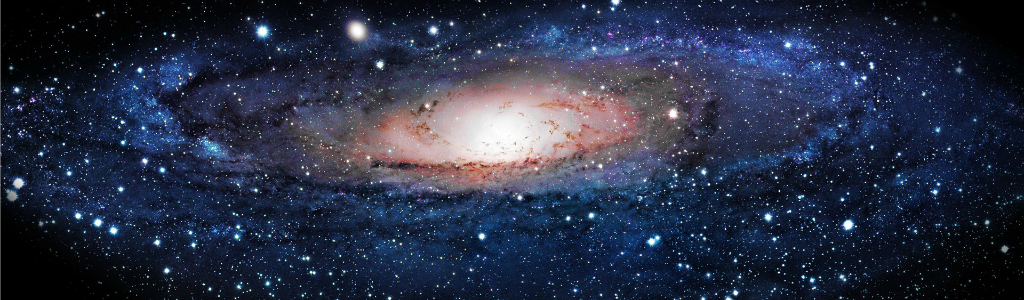
\includegraphics[width=11cm]{trou_noir}
    \label{fig:trou_noir}
\end{figure}


%%%----------------------------------------------------------
\chapter{Les suites}
%%%----------------------------------------------------------


Pour commencer qu'est-ce qu'une suite?

\begin{quote}[suites réelles]
  Une suite réelle est une liste indexée de nombres réels. \\
  On appelle suite réelle tout application de $\N$ dans $\R$: 
  $
  u
  \left\{
  \begin{array}{rcl}
    \N  & \longrightarrow  	& \R \\
    n  	& \longmapsto   	& u_n \\
  \end{array}
  \right.
  $\\
\end{quote}

Nous pouvons aussi parler de suites numériques:

\begin{quote}[suites numérique]
  Une suite numérique est une liste indexée de nombres.\\ 
  Si les nombres sont réels on parle de suite réelle. 
  Si les nombres sont complexes on parle de suite complexe.\\
  Une suite   
  $
  \begin{array}{rcl}
   u_n
  \end{array}
  $ multipliée par 10 est définie comme une suite de \textbf{\textit{raison}} 10.
\end{quote}


Une des suites les plus célèbres est la suite de \textbf{Fibonacci}.

Cette suite doit son nom au mathématicien Leonardo Pisano Fibonacci (v. 1175 – v. 1250) qui avec des lapins a pu en déduire une formule récursive.  Ce mathématicien s’est demandé quelle serait la population de lapins à un mois donné en supposant qu’un couple de lapereaux doit attendre un mois avant de donner naissance à un autre couple. Par exemple :

\begin{itemize}
    \item Mois 1: un couple de lapeaux (A) \begin{math}\rightarrow\end{math} 1 couple
    \item Mois 2 : Un couple de lapins (A) \begin{math}\rightarrow\end{math} 1 couple
	\item Mois 3 : Un couple de lapins (A) et un couple de lapereaux (B) \begin{math}\rightarrow\end{math} 2 couples
	\item Mois 4 : Deux couples de lapins (A et B) et un couple de lapereaux (C qui vient du couple A) \begin{math}\rightarrow\end{math} 3 couples
	\item Mois 5 : 3 couples de lapins (A, B, C) et 2 couples de lapereaux (D venant de A, E venant de B) \begin{math}\rightarrow\end{math} 5 couples
	\item Mois 6 : 5 couples de lapins (A, B, C, D, E) et 3 couples de lapereaux \begin{math}\rightarrow\end{math} 8 couples
	\item Mois 7 : 8 couples de lapins et 5 couples de lapereaux \begin{math}\rightarrow\end{math} 13 couples
	\item Mois X: ... \\
\end{itemize} 


Cette suite de nombres (1, 1, 2, 3, 5, 8, 13...) est donc la suite de Fibonacci.
Nous pouvons remarquer que si nous additionnons les deux derniers nombres otenus de la suite, nous obtenons le nombre suivant \textit{(M = Mois)}:

\begin{itemize}
    \item 1 (M1) + 1 (M2) = 2 (M3)
    \item 1 (M2) + 2 (M3) = 3 (M4)  
    \item 2 (M3)  + 3 (M4) = 5 (M5) \\
\end{itemize}

Cette suite de \textit{Fibonacci} peut être représentée sous forme d'arbre:
\begin{figure} [!h]
    \centering
    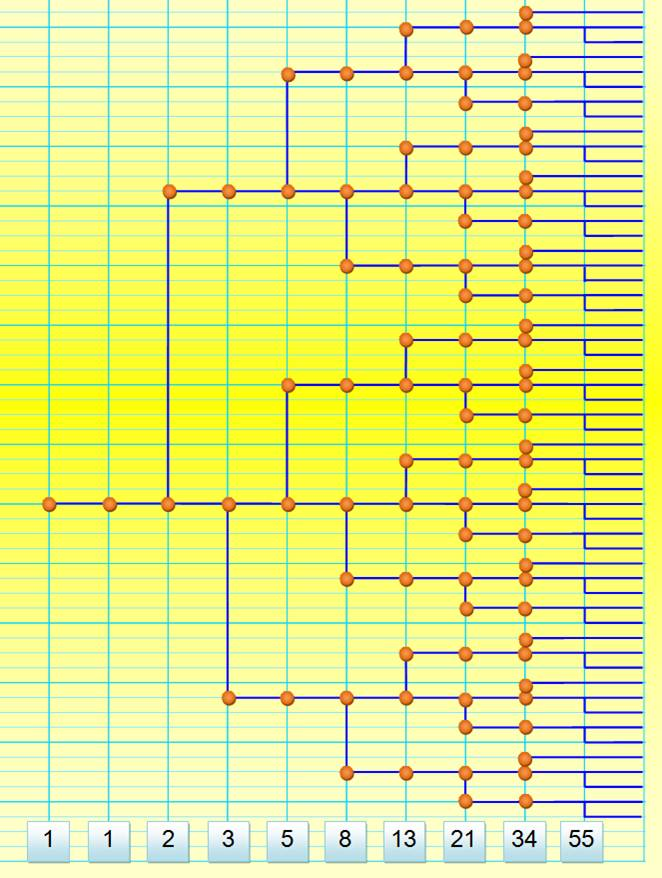
\includegraphics[width=9cm]{arbre_fibo}
    \label{fig:arbre_fibo}
    \caption{Suite de Fibonacci}
\end{figure}

Voici maintenant une implémentation de cette suite sous python:


\begin{lstlisting}[language=python]
    def fibonacci(n):
	# computation from definition of a Fibonacci number
	if n == 0:
		return 0
	if n == 1:
		return 1
	F_n_2 = 0
	F_n_1 = 1
	for k in range(n - 1):
		F_n = F_n_1 + F_n_2
		F_n_2 = F_n_1
		F_n_1 = F_n
	return F_n
\end{lstlisting}

Ceci clos le chapitre sur les suites


%%%----------------------------------------------------------
\chapter{Le chaos}
%%%----------------------------------------------------------

Nous savons maintenant ce qu'est une suite, passons donc à ce qui nous intéresse plus particulièrement: le \textbf{chaos}.
Derrière ce mot effrayant se cache une réelle théorie, la dénommée \textit{Théorie du Chaos}.
Qu'est-ce que cette théorie et qu'est-ce que le chaos?


Les théories du Chaos permettent de mettre un nom sur un ordre caché dans un apparent désordre. Avant l’apparition de ces théories et des ordinateurs, on ne pouvait calculer que des phénomènes linéaires (comme avec la suite de Fibonacci) car c’était considéré comme trop complexe. En réalité chaque système qui semble chaotique découle des propriétés d’une fonction bien précise. 

Une fonction est dite chaotique si elle présente les caractéristique suivantes:
\begin{itemize}
    \item Une sensibilité aux conditions initiales
    \item Un phénomène écrit par des équations différentielles
    \item On sent une forte récurrence
    \item C’est attiré vers un point attracteur ayant dans beaucoup de cas une dimension fractale (nous y reviendrons plus tard)
    \item Le comportement du système n’est pas le même que le comportement temporel. \\
\end{itemize}


Pour pouvoir continuer, on a besoin de définir ce qu’est un point attracteur. Comme son nom l’indique c’est tout simplement un point qui semble attirer tout ce qui est autour, tel le centre d’un trou noir.

Utilisons le code suivant:
\begin{lstlisting}[language=python]
f(x) = 4*x*(1-x)

def liste_suite(f,terme_init,n):
	maliste = []
	x = terme_init
	for k in range(n):
		maliste.append(x)
		x = f(x)
	return maliste


def liste_points(f,terme_init,n):
	u = liste_suite(f,terme_init,n)
	mespoints = [ (u[0],0) ]
	for k in range(n-1):
		mespoints.append( (u[k],u[k+1]) )
		mespoints.append( (u[k+1],u[k+1]) )
	return mespoints

def dessine_suite(f,terme_init,n):
	mespoints = liste_points(f,terme_init,n)
	G = plot(f,(x,0,1), color='red') # La fonction
	G = G + plot(x,(x,0,1), color='green') # La droite (y=x)
	G = G + line(mespoints) # La suite
	G.show()

dessine_suite(f,0.123,100)
\end{lstlisting}

Lorsqu'on regarde cette image obtenue avec le code précédent 
\begin{figure} [!h]
    \centering
    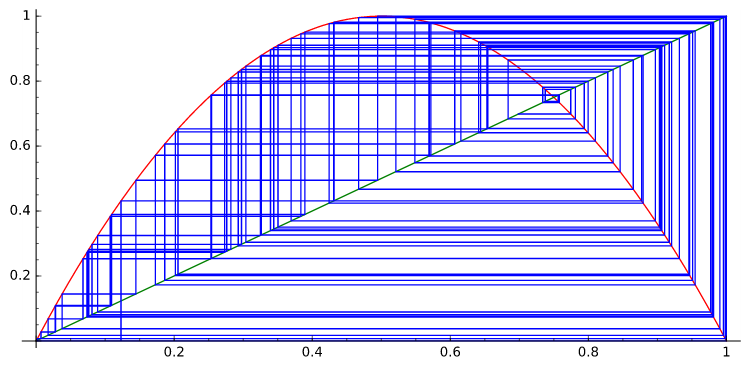
\includegraphics[width=8cm]{chaos}
    \label{fig:chaos}
    \caption{Chaos}
\end{figure}

on s'imagine qu'il n'y a aucun lien possible possible entre quoi que ce soit, qu'aucune fonction logique ne peut en arrriver là. C'est pourtant faux var cette image réagit à la fonction 
\begin{lstlisting}
    f(x) = r*x*(1-x)
\end{lstlisting}
. De plus, cela réagit au nombre \textit{r} qui, lorsqu'il augmente, rend la fonction encore plus chaotique (ici \textit{r} vaut \textit{4}).
Par rapport aux caractéristiques précédemment définis, on peut dire que la fonction est sensible aux conditions initiales (si on fait évoluer une condition alors la fonction change totalement), la fonction est écrite par une équation, il y a une forte récurrence, c’est attiré vers un point attracteur (ici situé en (0,68;0;78) approximativement, le point étant l'intersection entre deux autres fonctions) et le comportement n’est pas « normal ».


Autre exemple, celui de la bifurcation. On obtient une bifurcation avec 
\begin{lstlisting}[language = python]
    f(x,r) = r*x*(1-x)
    
    def bifurcation(F,terme_init):
    Nmin = 100 # On oublie Nmin premiers termes
    Nmax = 200 # On conserve les termes entre Nmin et Nmax
    epsilon = 0.005 # On fait varier r de epsilon à chaque pas
    r = 2.5 # r initial
    mespoints = []
    while r <= 4.0:
        u = liste_suite(F(r=r),terme_init,Nmax) # On calcule la suite
        for k in range(Nmin,Nmax):
            mespoints = mespoints + [(u[k],r)]
        r = r + epsilon
    G = points(mespoints)
    G.show()
    
    bifurcation(f,0.102)
\end{lstlisting}
et lorsqu’on augmente le paramètre \textit{r}, on obtient une succession de bifurcations entre les comportements périodiques et le chaos.
\begin{figure} [!h]
    \centering
    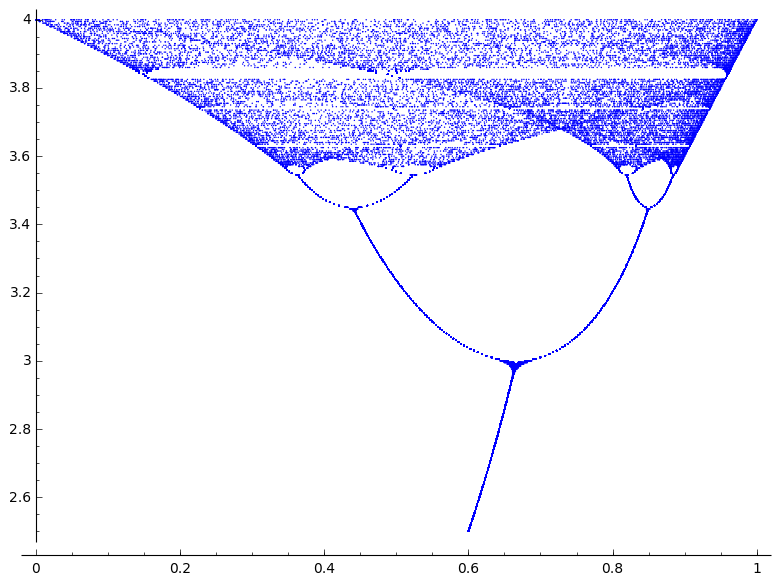
\includegraphics[width=6cm]{bifurcation}
    \label{fig:bifurcation}
    \caption{Bifurcation}
\end{figure}

Sur l'image précédente nous pouvons voir:
\begin{itemize}
    \item Pour 0 < \textit{r} < 3 , le système possède un point fixe attractif, qui devient instable lorsque \textit{r} = 3
    \item Pour 3 \begin{math}\le\end{math} \textit{r} < 3,67 , l'application possède un attracteur qui est une orbite périodique, de période     
    \begin{math} 2^n 
     \end{math} où n est un entier qui tend vers l'infini lorsque \textit{r} tend vers 3.57
    \item Lorsque \textit{r} = 3.57..., l'application possède un attracteur chaotique fractal découvert par le biologiste \textit{May} en 1967
\end{itemize}

Lorsque le paramètre \textit{r} augmente, on obtient donc une succession de bifurcations entre les comportements périodiques et le chaos, résumée sur la figure ci-contre.
Comme vous avez pu le remarquer j’ai cité plusieurs fois le mot \textit{fractale}, mais qu’est-ce que cela ?



%%%----------------------------------------------------------     
\chapter{Les fractales}
%%%----------------------------------------------------------

Fractale vient du mot « fraction » de ce fait on peut s’imaginer qu’avec tout ça il va y avoir une histoire de division.

Sur une figure normale, lorsqu’on zoome sur n’importe quel point sur celle-ci alors on aura tendance à voir une ligne droite. Sur une fractale c’est l’inverse. Lorsqu’on zoom sur un point quelconque, on voit au fur et à mesure apparaître de plus en plus de petits détails sans que cela ne s’arrête. On peut retrouver cela dans la vie de tous les jours comme avec la frontière de l’Angleterre. On voir que si l’on zoom de plus en plus à n’importe quel point de cette île, on voit que ce n’est pas lisse. Il y aura toujours un petit détail comme avec des falaises ou des rochers ou bien même des grains de sable. De ce fait on est en mesure de se demander combien mesurent les côtes anglaises. Le mathématicien \textit{Lewis Fry Richardson} se l’est posée et est arrivé à la conclusion que la longueur des côtes britanniques est de plus en plus grande lorsqu’on zoom dessus jusqu’à atteindre l’infini, comme avec la figure de Von Koch.
Cette figure est obtenue de la manière suivante:
\begin{itemize}
    \item On prend un segment de droite qu’on divise en 3 tiers
    \item On efface le segment du milieu
    \item A la place du trou laissé au milieu on ajoute 2 segments de longueur 1 tiers à chaque extrémité de ce trou (ce qui forme une sorte de triangle)
    \item On se retrouve avec une figure composée de 4 segments
    \item On répète ainsi ce procédé pour chaque segment de cette nouvelle forme (sur les segments qui correspondent au 1er tiers et au 3ème tiers ainsi que sur les 2 nouveaux côtés de la nouvelle forme triangulaire)
\end{itemize}

\vspace*{10mm}
Ce qui donne ceci: 
\vspace*{20mm}
\begin{figure} [!h]
    \centering
    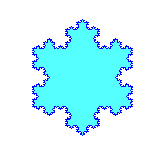
\includegraphics[width=6cm]{flocon}
    \label{fig:flocon}
    \caption{Flocon de Von Koch}
\end{figure}

Voici le code pour le faire apparaître (en utilisant un module \textit{Turtle} pour Python):

\begin{lstlisting}[language = python]
from turtle import * 
def floc(l) :
  if l<3 :
    fd(l)
    return
  floc(l/3) #dessiner le premier trait du triangle
  lt(60) #tourner le dessin
  floc(l/3) #dessiner le second trait du triangle, le cote gauche
  rt(120)
  floc(l/3) #dessiner le troisieme trait du triangle, le cote droit
  lt(60)
  floc(l/3) #dessiner le dernier trait du triangle
 
def flocon(l)  :
  speed(0)
  color('#0000ff', '#55ffff') # couleur du flocon
  begin_fill() #remplissage du flocon
  for i in range(3) :
    floc(l)
    rt(120)
  end_fill()
 
flocon(100)
\end{lstlisting}

Ces fractales servent de modèles pour décrire des phénomènes chaotiques.
Il existe 3 modèles de fractales : les objets fractals, les fractales déterministes et les fractales naturelles. 
Un \textbf{objet fractal} comme le flocon de Von Koch ou le tapis de Sierpinski (parfois appelé tamis de Sierpinski que l’on retrouve notamment dans le jeu Zelda sous le nom de Triforce) se définit comme des structures obtenues par itération d’un algorithme géométrique sur une figure, c’est-à-dire qu’on débute avec un objet graphique (comme un triangle) puis on définit une opération ou une série d’opérations qui va ajouter un élément à l’objet et en répétant cela à l’infini on obtient la naissance d’un objet fractal. 

\begin{figure} [!h]
    \centering
    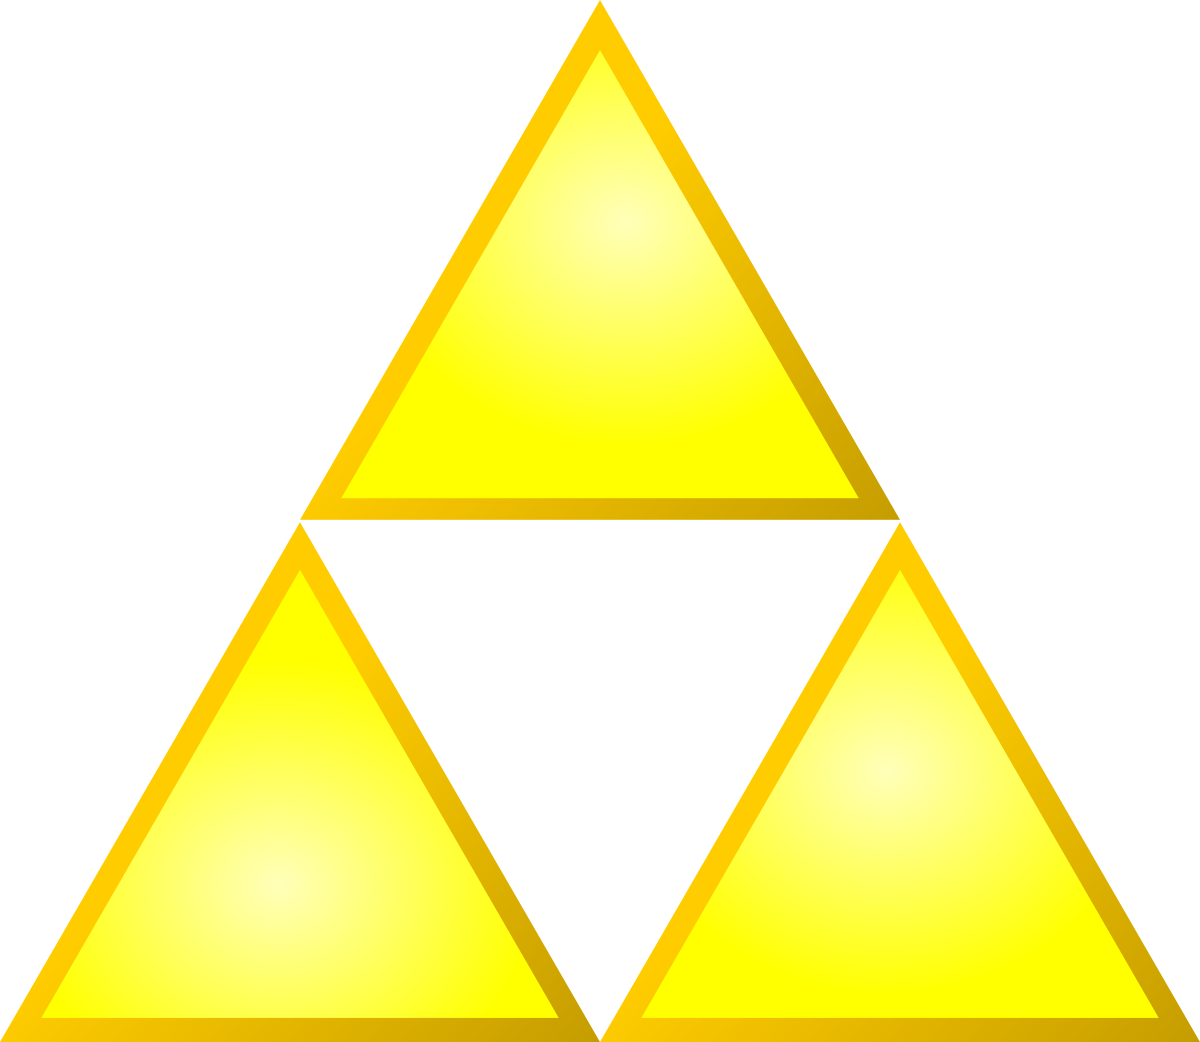
\includegraphics[width=6cm]{triforce}
    \label{fig:triforce}
    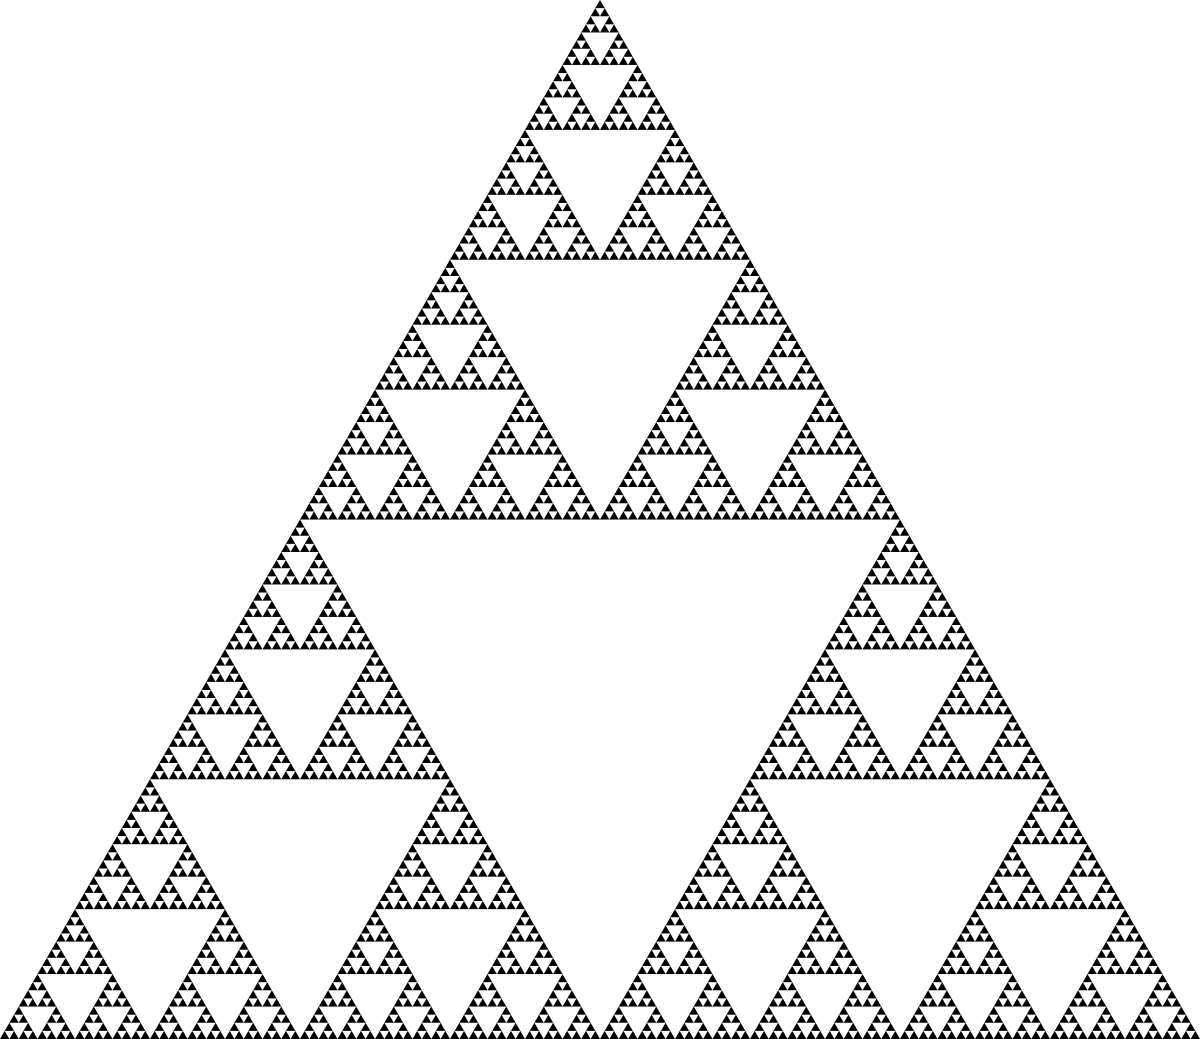
\includegraphics[width=6cm]{triangle_sierpinski}
    \label{fig:triangle_sierpinski}
    \caption{Le triforce et le triangle de Sierpinski}
\end{figure}

Nous avons ensuite les \textbf{fractales déterministes}. Nous n’allons pas beaucoup nous attarder sur ces dernières car elles sont plus complexes que les autres et elles utilisent beaucoup les mathématiques. En fractale déterministe nous avons par exemple l’ensemble de Mandelbrot ou les ensembles de Julia.
\vspace*{10mm}
\begin{figure} [!h]
    \centering
    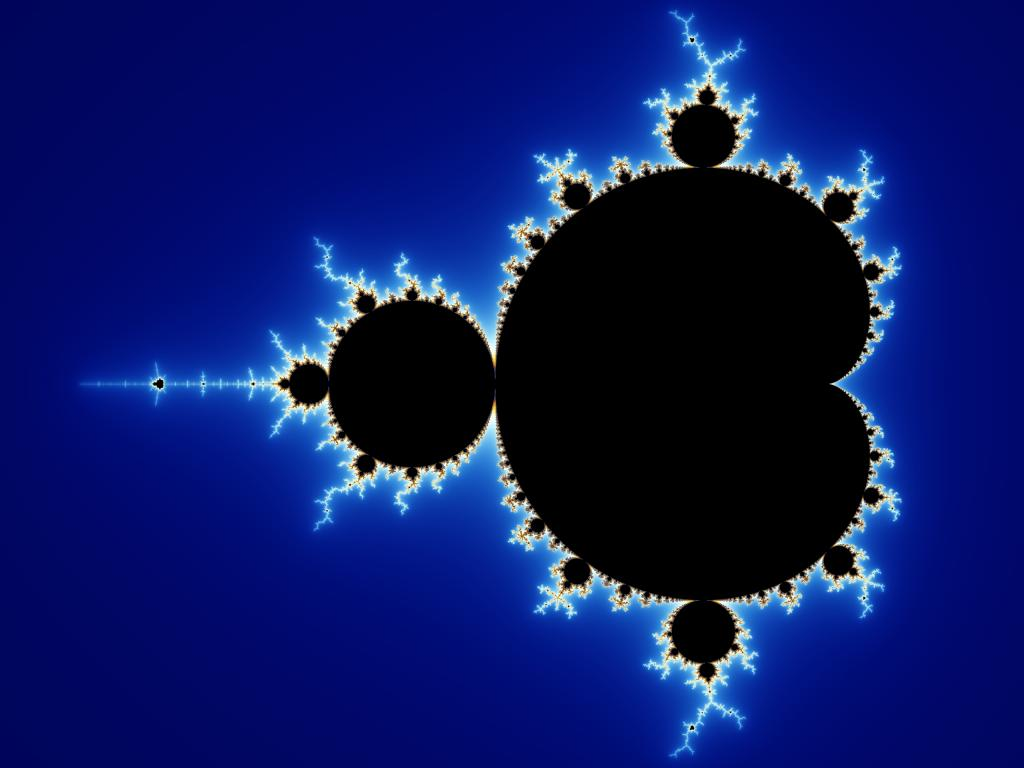
\includegraphics[width=7cm]{mandelbrot}
    \label{fig:mandelbrot}
    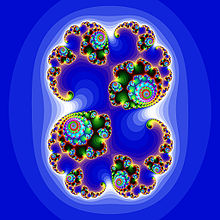
\includegraphics[width=7cm]{julia}
    \label{fig:julia}
    \caption{L'ensemble de Mandelbrot et les ensembles de Julia}
\end{figure}
\vspace*{10mm}

La troisième catégorie de fractales est la catégorie des \textbf{fractales naturelles}. Les arbres, les nuages et même les choux-fleurs sont des fractales naturelles. En effet on retrouve là-dedans un système qui se répète. Un exemple simple de fractale naturel est la fougère qui n’a pas une complexité infinie (elle s’arrête à la plus petite feuille de la fougère) mais c’est la preuve que les fractales existent bel et bien dans la nature et sans l’intervention de l’homme.
\vspace*{10mm}

\begin{figure} [!h]
    \centering
    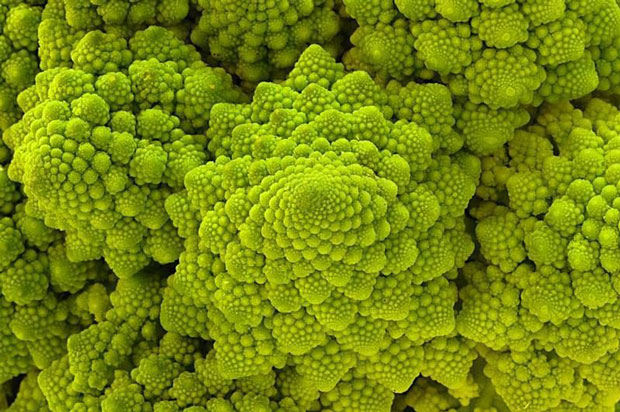
\includegraphics[width=6cm]{choux_fleur}
    \label{fig:choux_fleur}
    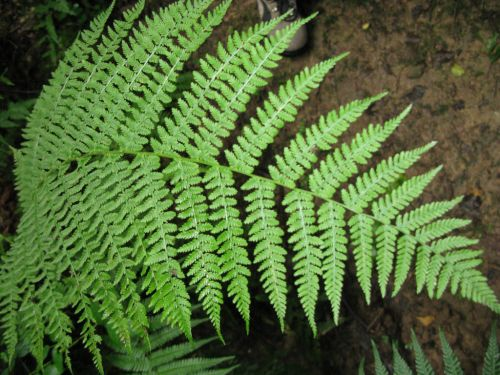
\includegraphics[width=6cm]{fougere}
    \label{fig:fougere}
    \caption{Des exemples de fractales naturelles}
\end{figure}

%%%----------------------------------------------------------
\chapter{Le lien entre la théorie du chaos et les fractales}
%%%----------------------------------------------------------

Pourquoi avoir fait ce crochet par les fractales me diriez-vous ? Et bien tout simplement à cause de réelles similitudes entre les deux !
Nous allons relever 3 points importants au niveau de la similitude entre le chaos et les fractales.

\begin{enumerate}
    \item Que nous prenons un objet fractal ou un phénomène chaotique, il est impossible de déterminer la valeur exacte d’un point en utilisant deux points autour de ce dernier, même si ceux-ci sont très proches du point que nous cherchons à déterminer.  Cela s’explique du fait que le point intermédiaire peut se situer n’importe où et que nous avons un caractère infini sur les fractales.
    Pour illustrer ce propos il suffit de prendre un phénomène chaotique naturel : l’écoulement d’un liquide. Lorsque l’on vide un évier nous pouvons remarquer un phénomène chaotique avec l’apparition de grands et petits tourbillons. Il est impossible de déterminer où se situe n’importe quel point, pouvant être sur un grand tourbillon ou bien même sur un petit tourbillon.
    \begin{figure} [!h]
    \centering
    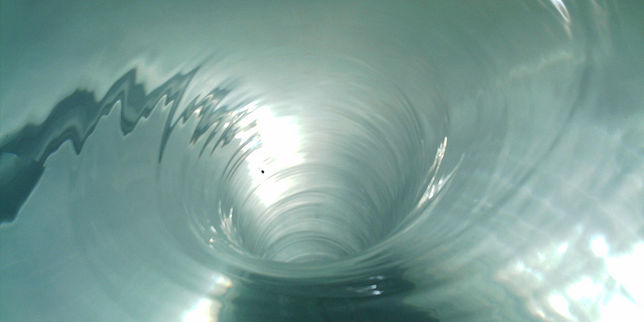
\includegraphics[width=6cm]{tourbillon}
    \label{fig:tourbillon}
    \caption{Le tourbillon de l'eau}
    \end{figure}
    \item La non-linéarité mais leur totale détermination. Pour résumer plus simplement, la forme des différentes équations linéaires semblent visuellement chaotique. En réalité, si l’on zoome, quelle que soit l’échelle où l’on inspecte, on y retrouvera des formes similaires : on appelle cela une symétrie d’échelle.
    \item La dernière similitude abordée est la plus abstraite, c’est l’évolution des phénomènes dans un espace de phase. Lorsqu’un système dépend d’un nombre x de variables, on peut déterminer un système de coordonnées avec une dimension pour chaque variable. A n’importe quel moment, le phénomène en question est représenté par un point dans l’espace déterminé précédemment et l’ensemble de tous ces points dessine une figure, figure qui s’appelle un attracteur.
    Dans le TP nous pouvons voir un attracteur qui se situe en un point donné qui est au croisement des deux fonctions.
    \begin{figure} [!h]
        \centering
        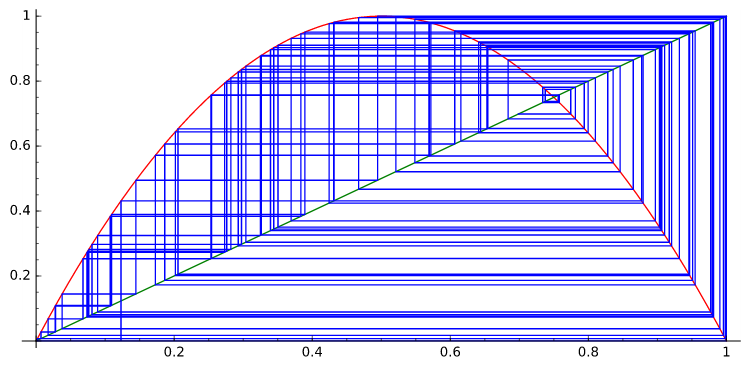
\includegraphics[width=8cm]{chaos}
        \label{fig:chaos}
        \caption{Chaos}
    \end{figure}

    Prenons un exemple simple : pour un pendule simple, l’attracteur est un cercle où l’un de ses axes de coordonnées représente la distance de l’extrémité par rapport à la verticale et l’autre axe représente sa vitesse à chaque instant.
    \begin{figure} [!h]
        \centering
        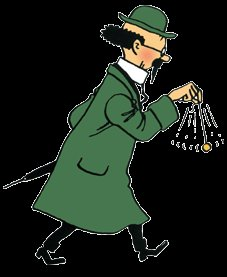
\includegraphics[width=6cm]{pendule_tournesol}
        \label{fig:pendule_tournesol}
        \caption{Le professeur Tournesol et son pendule}
    \end{figure}
    
    En revanche dans des systèmes chaotiques, l’attracteur devient plus complexe avec une trajectoire qui ne se recoupe jamais. 
    \begin{figure} [!h]
        \centering
        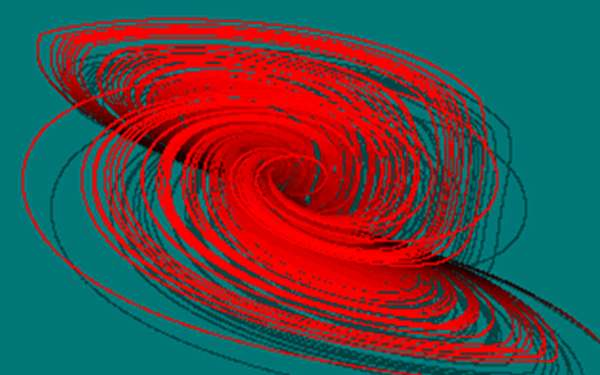
\includegraphics[width=6cm]{attracteur_complexe}
        \label{fig:attracteur_complexe}
        \caption{Un attracteur complexe}
    \end{figure}
    
    De ce fait, cet attracteur porte le nom d’attracteur étrange. Dans différents cas l’attracteur la structure de cet attracteur est fractal.
    Un des plus célèbres attracteurs étranges est l’attracteur de Rossler qui est associé a un système dynamique ayant 3 équations différentielles non-linéaires qui sont :
    
    \begin{equation}
        \frac{dx}{dt} = - y - x
    \end{equation}
    \begin{equation}
        \frac{dy}{dt} = x + a * y
    \end{equation}
    \begin{equation}
        \frac{dz}{dt} = b + z * (x - c)
    \end{equation}
    
    \begin{figure} [!h]
        \centering
        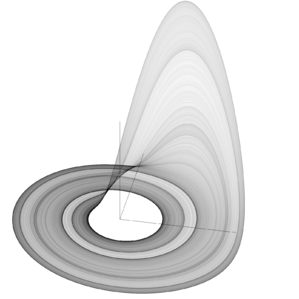
\includegraphics[width=6cm]{rossler}
        \label{fig:rossler}
        \caption{L'attracteur de Rossler}
    \end{figure}


\end{enumerate}


%%%----------------------------------------------------------
\chapter{Le nombre d'or}
%%%----------------------------------------------------------

Le nombre d’or est un nombre qui lie plusieurs domaines des mathématiques qui pourtant en apparence, n’ont aucun lien entre eux. En effet, ils utilisent le nombre d’or qui révèle les liens entre eux.
C’est un nombre qui possède la propriété suivante : si on le multiplie par lui-même, cela revient à lui ajouter 1. Si on fait 1,618… * 1,618… = 2,618… Même si on s’arrête ici aux 3 premières décimales, ce résultat est toujours exact à une infinité de décimales après la virgule.
La formule du nombre d’or est \begin{math}\frac{1 + \sqrt(5)}{2}\end{math}. Ce n’ombre d’or est plus communément appelé \begin{math}\phi\end{math} (PHI, lettre grecque). Donc \begin{math}\phi = \frac{1 + \sqrt(5)}{2} = 1,618… \end{math}\\


La propriété géométrique du nombre d’or est que si on prend un segment de longueur 1 (pour l’exemple) et qu’on le multiplie par PHI on obtient un nouveau segment dont la longueur est environ 1,618. On prend ensuite ce nouveau segment qu’on multiplie par \begin{math}\phi\end{math} et on obtient donc un nouveau segment dont la longueur est de \begin{math}\phi * \phi\end{math} c’est-à-dire environ 2,618. On peut donc dire que la somme des deux premiers segments est égale à la longueur du troisième segment \begin{math}\phi * \phi\end{math}. On peut partir de n’importe quel segment de départ et la somme des deux premiers segments sera toujours égale à la longueur du troisième.\\

L’histoire du nombre d’or débute dans l’antiquité grecque. Ce nombre est surtout utilisé à des fins esthétiques faites par l’homme mais peut également se trouver dans la nature comme avec les étamines d’un tournesol ou en comptant le nombre de spirales qu’il y a sur un ananas.\\

\vspace*{35mm}

\begin{figure} [!h]
    \centering
    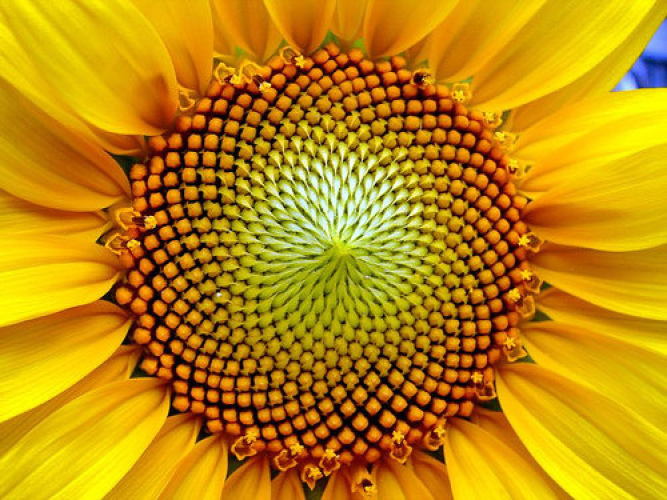
\includegraphics[width=6cm]{tournesol}
    \label{fig:tournesol}
    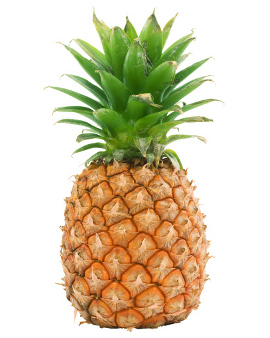
\includegraphics[width=5cm]{ananas}
    \label{fig:ananas}
    \caption{Les étamines d'un tournesol et un ananas}
\end{figure}

Avec le nombre d’or on associe souvent le rectangle d’or qui est un rectangle dont la longueur est PHI fois plus grande que la largeur. La propriété principale du rectangle d’or est que si on dessine un carré sur une de ces longueurs on obtient un rectangle plus grand qui est lui aussi un rectangle d’or. Par exemple on prend un rectangle de largeur 1 et de longueur \begin{math}\phi\end{math} alors le nouveau rectangle a une largeur égale à \begin{math}\phi\end{math} et a une longueur égale à \begin{math}1 + \phi\end{math}, qui est égal à \begin{math}\phi * \phi\end{math} d’après la propriété du nombre d’or. On peut répéter ce processus une infinité de fois mais on peut aussi le faire dans le sens inverse. Dans le rectangle de base on trace un carré et de ce fait on obtient un rectangle d’or qui est plus petit. De même on peut le répéter à l’infini.\\

Le plus intéressant est que si dans chacun des carrés obtenus on dessine un quart de cercle, on obtient une spirale qui peut se prolonger dans l’infiniment grand comme dans l’infiniment petit. Cette spirale est appelée la spirale d’or.
\vspace*{60mm}
\begin{figure} [!h]
    \centering
    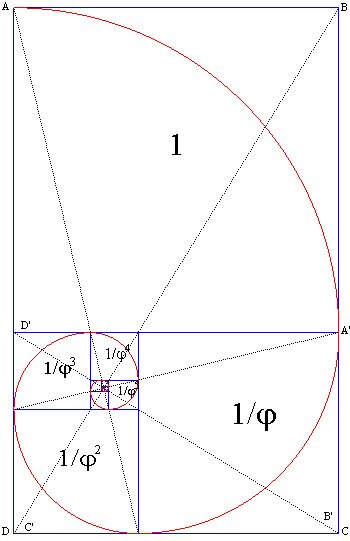
\includegraphics[width=9cm]{spirale_or}
    \label{fig:spirale_or}
    \caption{La spirale d'or et le rectangle d'or}
\end{figure}


Sur cette image, les nombres sont les côtés des carrés. Le rectangle d’or est considéré comme le rectangle le plus parfait esthétiquement par certains artistes.\\

Pourquoi parler du nombre d’or diriez-vous ? Et bien le nombre d’or intervient dans la suite de Fibonacci vue précédemment ! Souvenez-vous avec les couples de lapins… 
Le rapport entre le nombre d’or et la suite de Fibonacci est que la suite de Fibonacci permet de donner de très bonnes approximations du nombre d’or.  Pour rappel, les premiers termes de la suite de Fibonacci sont : 1, 1, 2, 3, 5, 8, 13, 21, 34… Si on fait le rapport de deux nombres consécutifs dans cette suite de Fibonacci, on tombe sur un nombre qui est proche du nombre d’or. Par exemple, \begin{math}\frac{13}{8}\end{math} donne 1,625, qui n'est pas très loin de 1,618. Plus on va loin dans la suite de Fibonacci, plus la précision va être bonne. Pour exprimer cela, on va utiliser le rectangle d’or.\\

Si on part d’un carré \begin{math}1 * 1\end{math} (les 2 premiers termes de la suite de Fibonacci), on lui ajoute un petit carré qui le fait se transformer en rectangle de taille \begin{math}1 * 2\end{math} (deux nombres consécutifs de la suite), puis on continue le processus et on a un rectangle de taille\begin{math}2 * 3\end{math}, puis un rectangle de taille \begin{math}3 * 5\end{math} puis \begin{math}5 * 8\end{math}… C’est une construction identique à celle du nombre d’or.
Le nombre d’or est donc impliqué dans tous les domaines où on retrouve la suite de Fibonacci, comme lorsqu’on compte le nombre de spirales d’un ananas nous allons trouver des termes de la suite de Fibonacci. 



%%%----------------------------------------------------------
\chapter{Conclusion}
%%%----------------------------------------------------------

Pour parler de chaos on peut penser à l’effet papillon. Pour voir cet effet papillon il est plus simple de considérer une fractale. En effet il y a une absence de frontière, que ce soit au plus petit ou au plus grand, avec la fractale on peut voir l’instabilité du comportement d’un système chaotique. C’est pour cela qu’on a défini que le battement d’aile d’un papillon pourrait modifier radicalement l’avenir climatique, voire créer un ouragan. Si on prend le modèle chaotique on peut voir qu’il s’applique bien et qu’il y a une limite de prévisibilité. D’un autre côté nous avons des modèles numériques qui montrent que ce n’est pas scientifique de pouvoir affirmer cela car l’énergie d’un papillon sera dissipé avant d’avoir pu produire un effet d’aussi grande amplitude. Tout cela peut aussi se retrouver dans les prévisions océaniques ou avec un phénomène perturbateur qui peut déclencher une avalanche.\\

Entre les fractales, les systèmes chaotiques et le nombre d’or nous pouvons voir quelques connexions :
\begin{itemize}
    \item Les dimensions de certaines fractales peuvent être proches du nombre d’or 
    \item Les structures répétitives conçues sur la proportion d’or comme avec le rectangle d’or ou la spirale d’or ou encore la suite de Fibonacci affichent une propriété d’autosimilarité qui les fait se focaliser sur leur centre
    \item Une modification même infime des conditions initiales peut être considérablement amplifiée par les structures répétitives construites sur le nombre d’or mais pas sur un caractère infini comme dans le cas du vrai chaos.
\end{itemize}

\begin{figure} [!h]
    \centering
    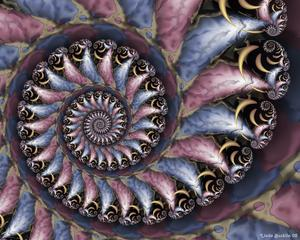
\includegraphics[width=6cm]{structure_or}
    \label{fig:structure_or}
    \caption{Les dimensions de cette fractales sont proches du nombre d'or}
\end{figure}

La suite de Fibonacci peut donc provoquer le chaos!

\begin{figure} [!h]
    \centering
    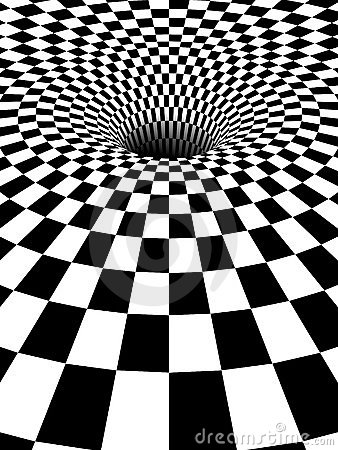
\includegraphics[width=6cm]{chaos2}
    \label{fig:chaos2}
    \caption{Le chaos...}
\end{figure}


\chapter{Commentaires}

Les suites et le chaos ont un lien très étroit même si cela n'es tpas évident à première vue. Travailler sur ce projet nous aura permis d'en apprendre plus sur tout cela, y compris les fractales.

\vspace*{40mm}

\begin{figure} [!h]
    \centering
    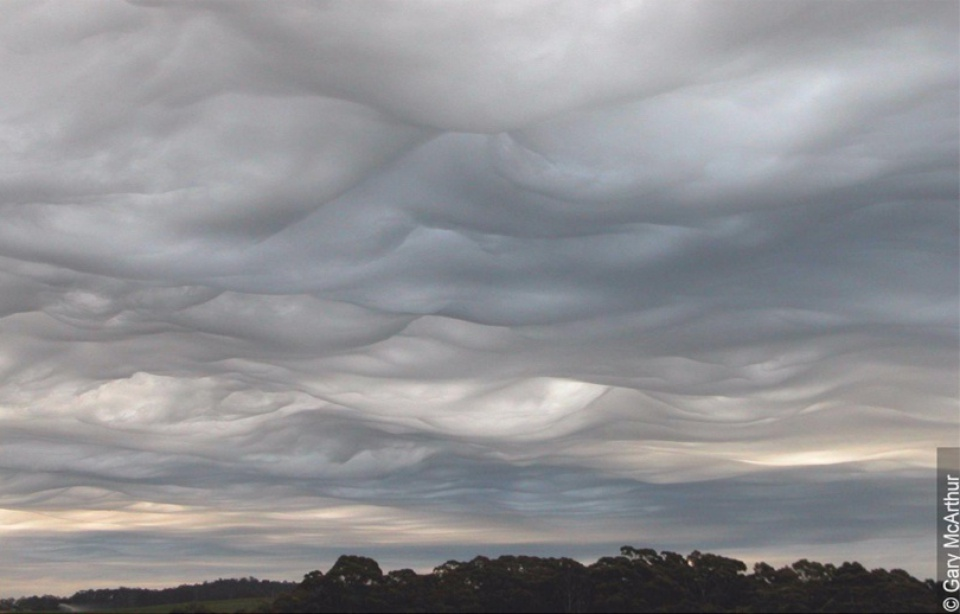
\includegraphics[width=11cm]{nuages}
    \label{fig:nuages}
    \caption{Des nuages aux allures de vagues chaotiques...}
\end{figure}


\end{document}
